% coming soon


The implementation of the continual planning and switching parts is
based on MAPSIM \cite{brenner:nebel:jaamas09} and is able to use
several planners as the underlying planning system. We use a modified
version of Fast Downward \cite{fast-downward}, which we extended with
the support for actions with success probabilities. Finally, we use
\system{dlib-ml} \cite{king:2009} for successive estimation of the
underlying belief-state.

The baseline approach is using the same continual planning system as
the switching planner, but instead of creating an observation problem
for the decision theoretic planner it will just execute one sensing
action -- assuming that this action will confirm its assumption.

To test our approch we use a robot exploration domain similar to the
one used on a physical robotic system. It involves a robot exploring
an office or living environment and trying to return objects to their
owner.

The basic building blocks of the domain consist of {\tt rooms}, {\tt
places} and {\tt objects}. Places are grouped in rooms and objects (as
well as the robot) are always in a place. The robot can move around
the rooms via connections between places given by the {\tt connected}
predicate. Each room has a (possibly unknown) {\em category/}
(e.g. kitchen, office, living room) and depending on this category,
objects are placed inside the rooms. An instance of this domain is
shown in figure\ref{fig}.

The robot can find out if an object is at a certain place by executing
the {\tt look-for-object} action, which may result in a perception if
the object is in fact there (though some objects are harder to detect
than others -- so absence of a percept is no proof of the object's
absence). Additionally, if the robot is in the presence of a human, it
may simply ask what type of room they are currently in -- but
conducting a dialogue is a bit more costly than simply running the
vision algorithm (cost of 8 vs costs of 3).

We conducted experiments on scenarios of several sizes with several
kinds of goals (though the goal is always reporting the position of a
certain kind of object). In order to determine the impact of sensor
reliability on both approaches, we also ran several tests in identical
problems with different probabilities for sensing the goal object. The
perception probabilities were 0.9, 9.65 and 04. As the initial state
of the problems is stochastic, we ran 50 simulations for each
configuration. The samples for the true initial state were drawn from
the same distribution that was used for planning, so the planner's
model matched its simulated world exactly. Not all problems generated
in this manner have a solution. We did not reject these problems, as
we believe that detecting the non-existance of a solution is as valuable
in exploration problems than finding one.

Fast Downward was run with the cyclic causal graph heuristic using A*
search or weighted A* with a weight of 5, depending on the difficulty
of the problem. We then performed multiple tests with different limits
for the belief space size of the decision theoretic subtask. Higher
limits should cause longer planning times but be beneficial to plan
quality as more contingencies can be taken in to account by the POMDP
planner.

\begin{figure}[h!]
  \centering
  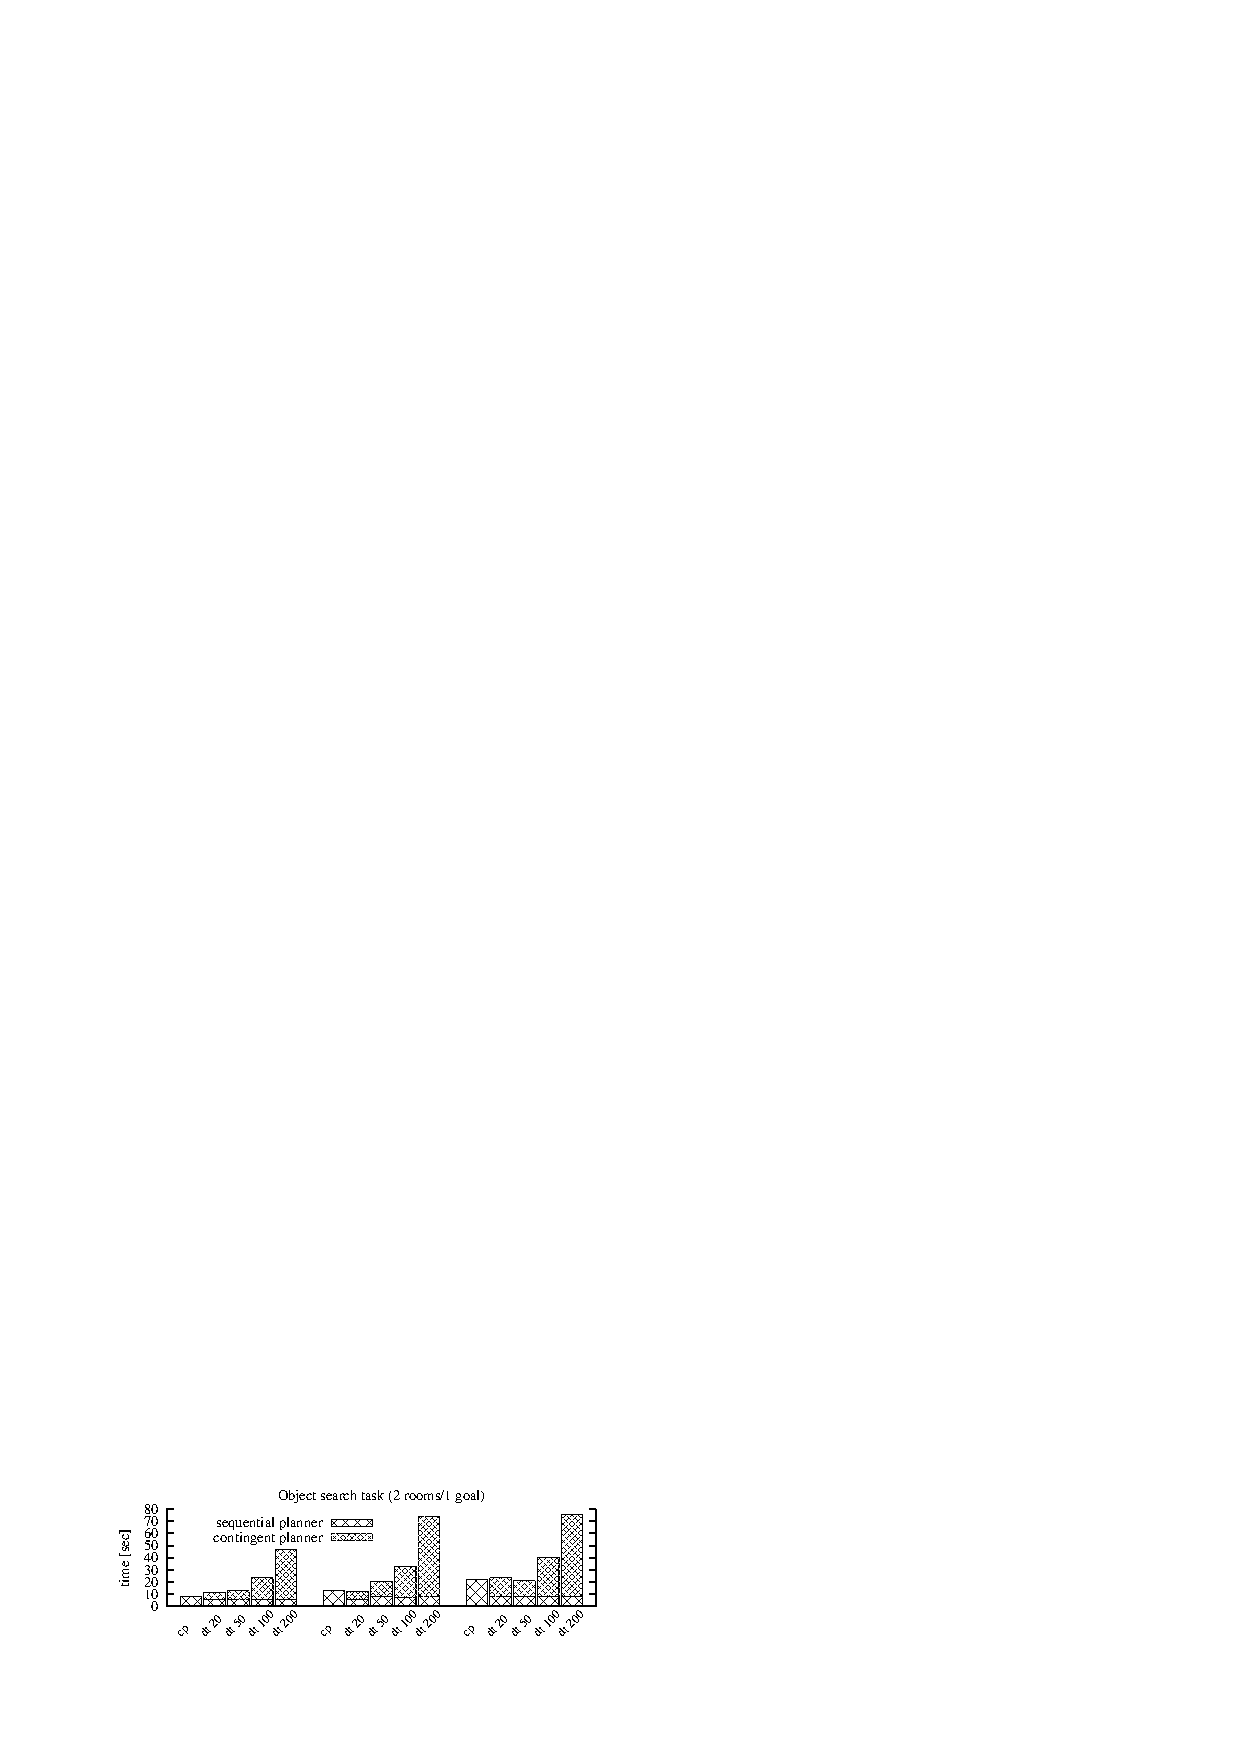
\includegraphics{dora1-time}
  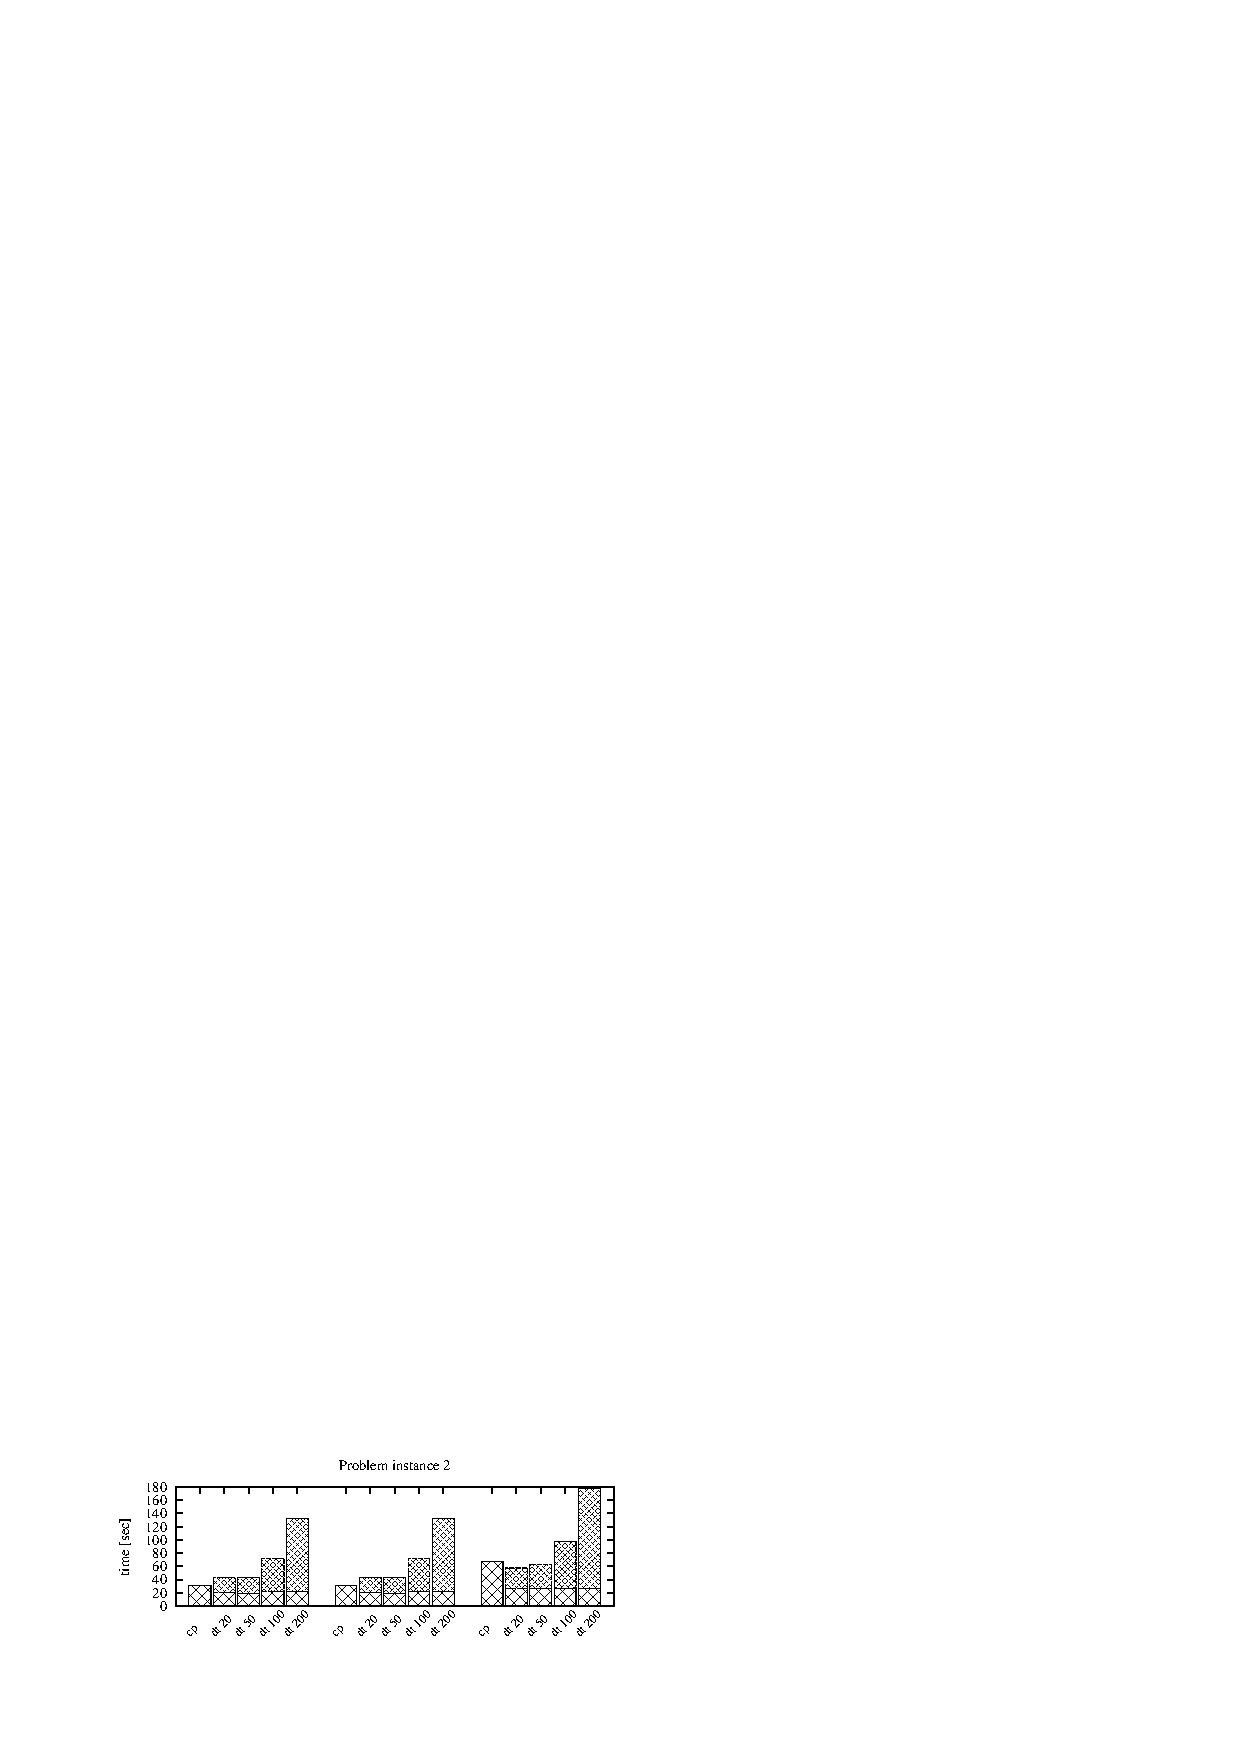
\includegraphics{dora2-time}
  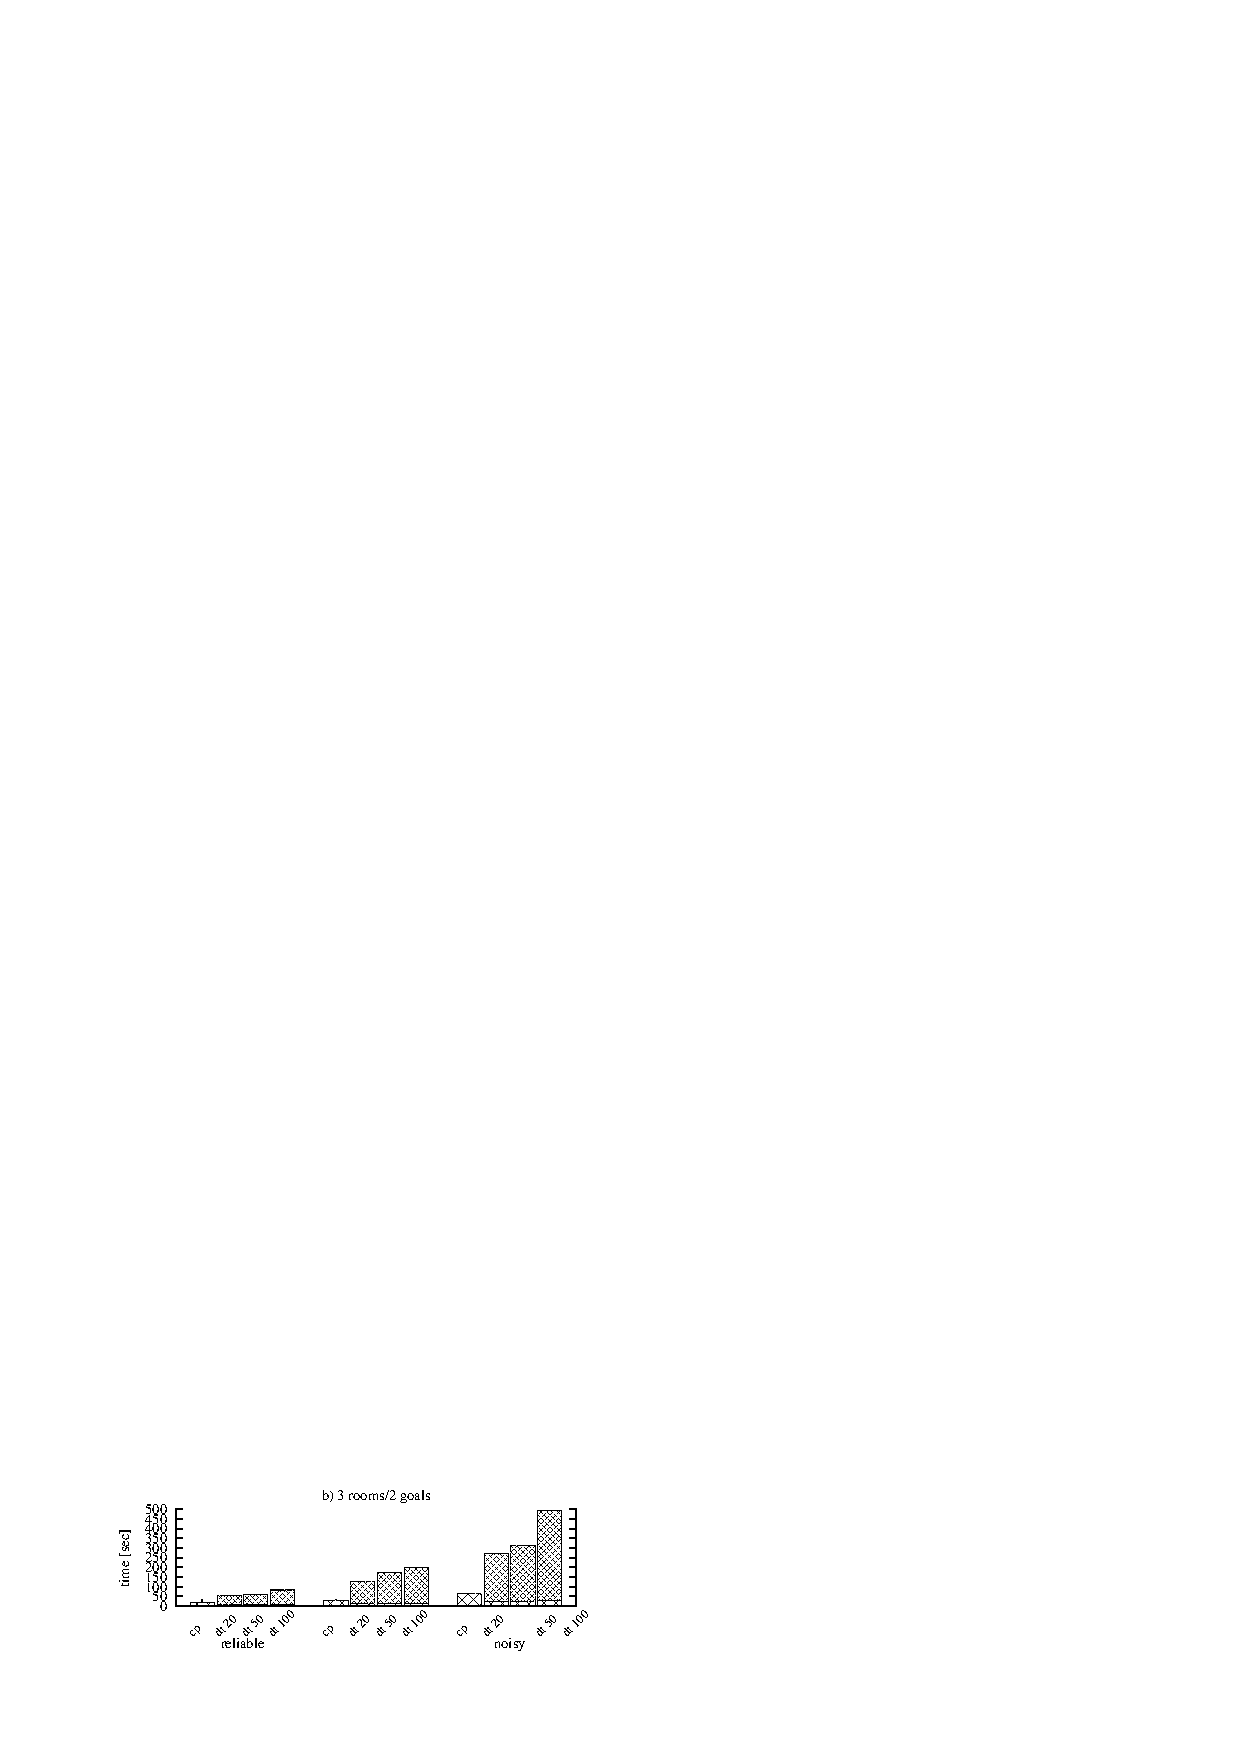
\includegraphics{dora3-time}
  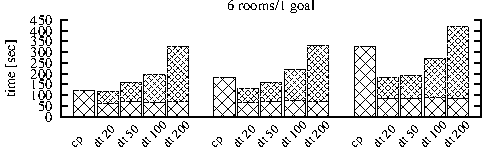
\includegraphics{dora4-time}
  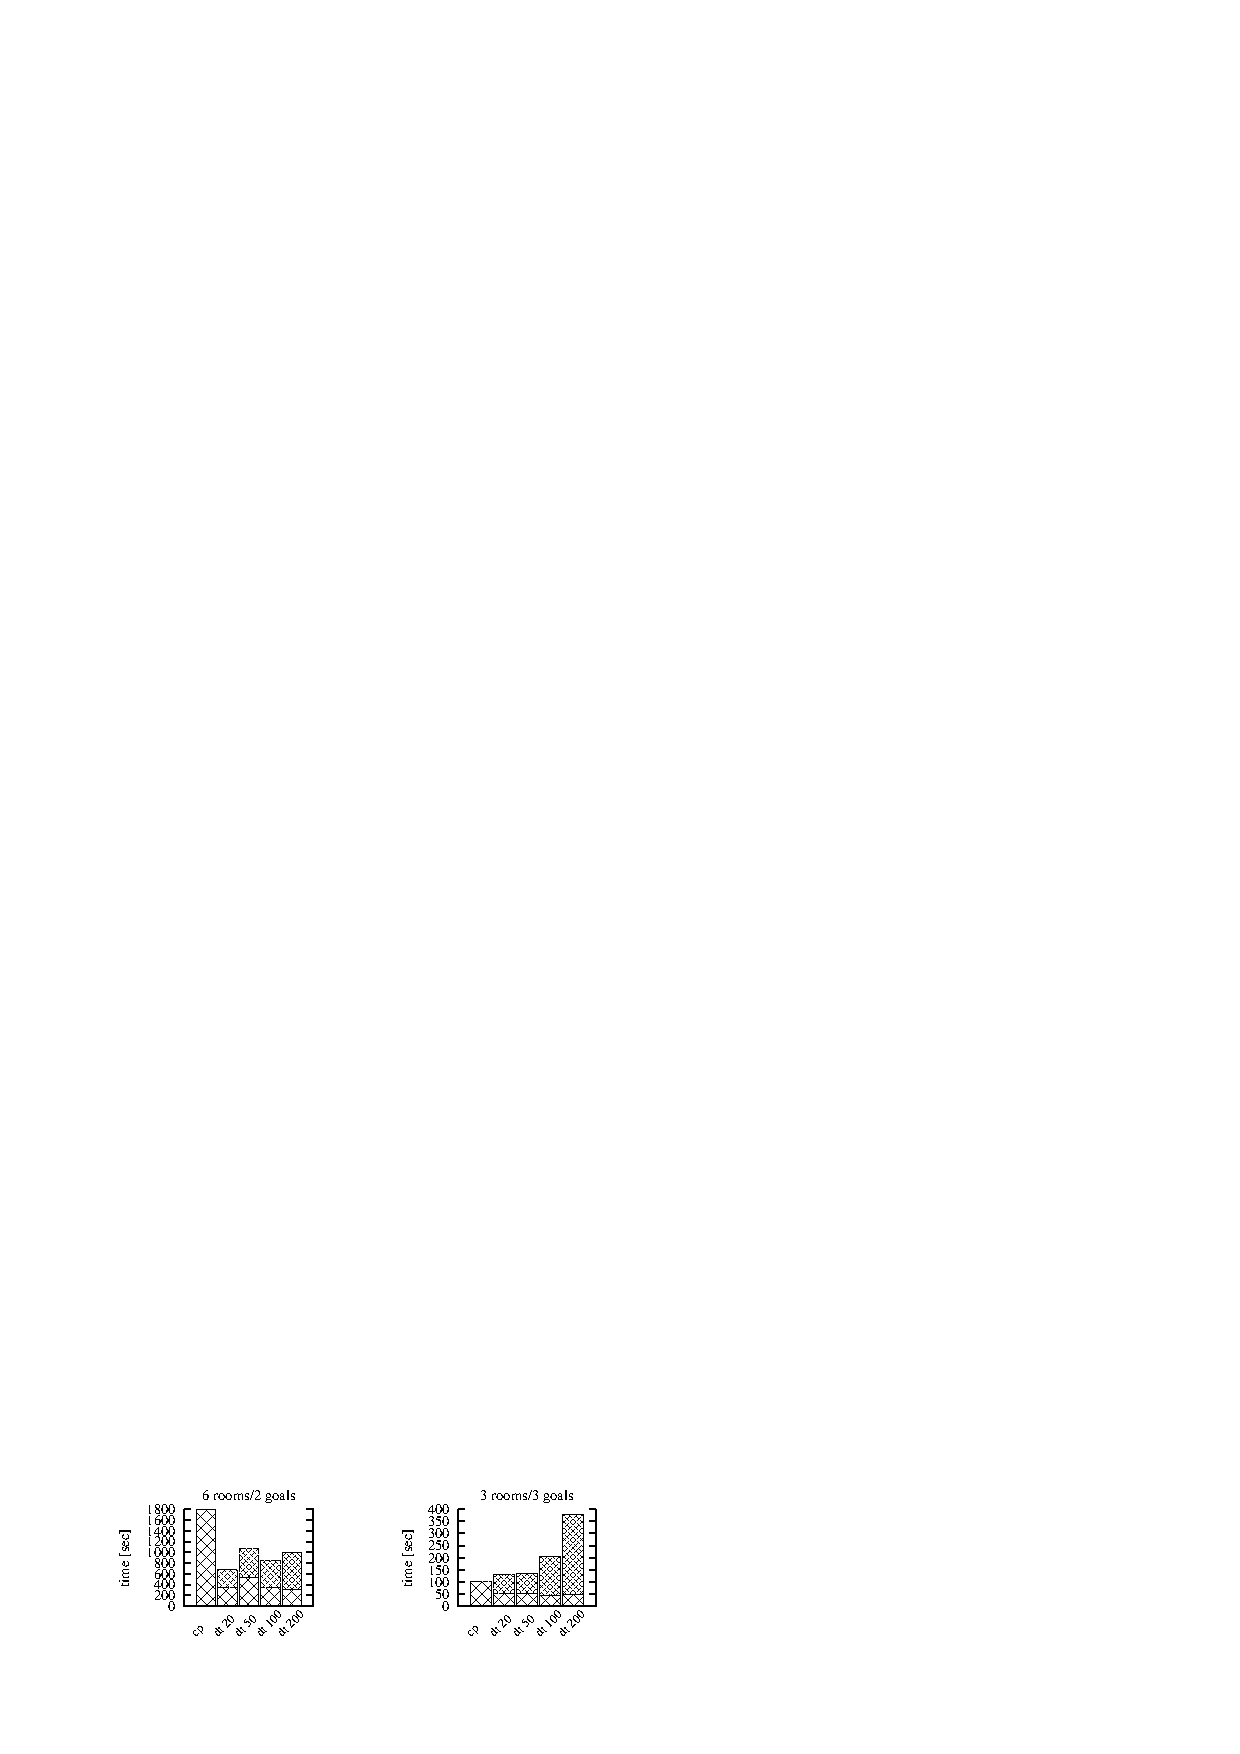
\includegraphics{dora56-time}
  \caption{Average runtime}
  \label{fig:results-time}
\end{figure}

\begin{figure}[h!]
  \centering
  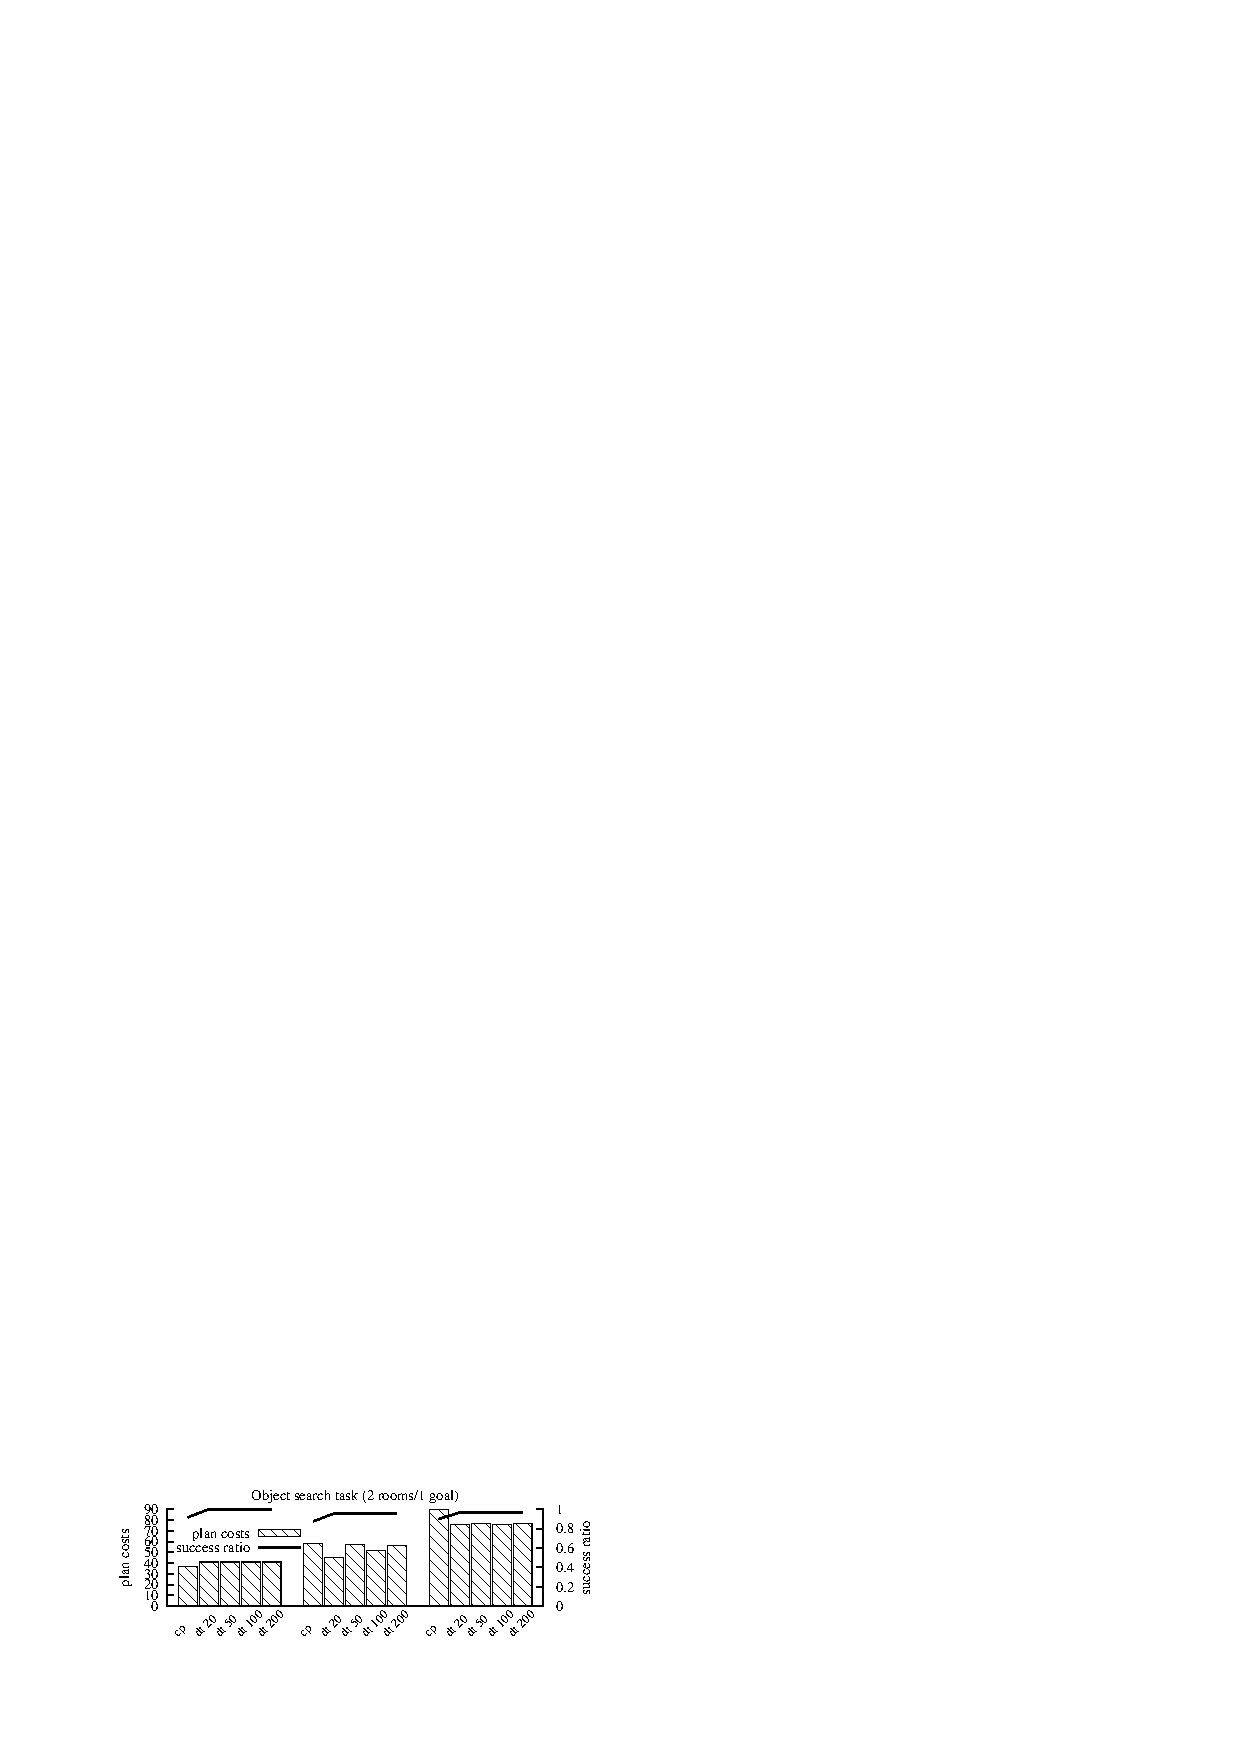
\includegraphics{dora1-quality}
  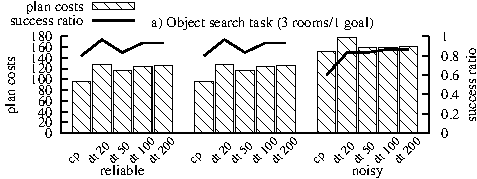
\includegraphics{dora2-quality}
  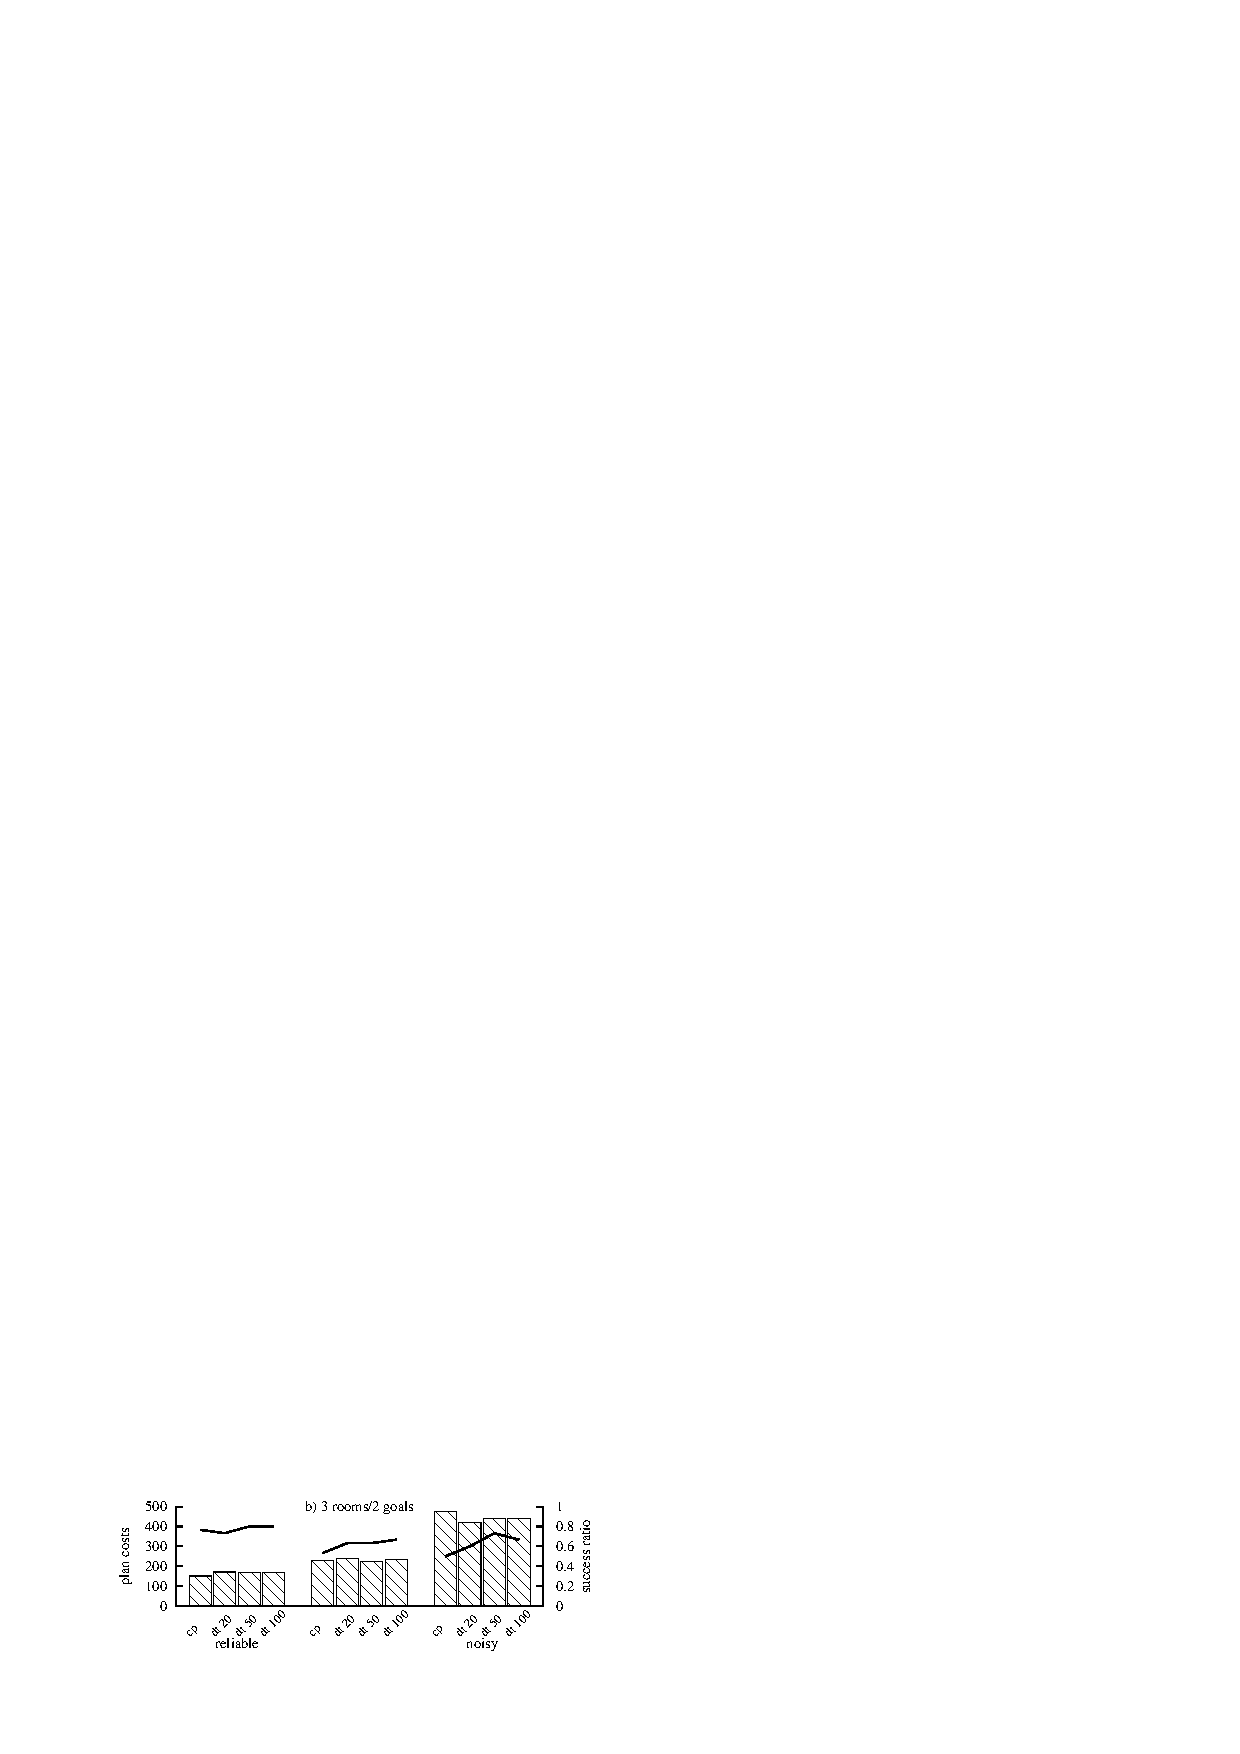
\includegraphics{dora3-quality}
  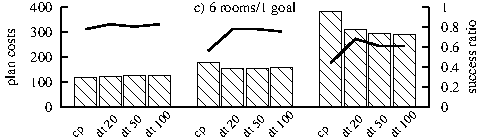
\includegraphics{dora4-quality}
  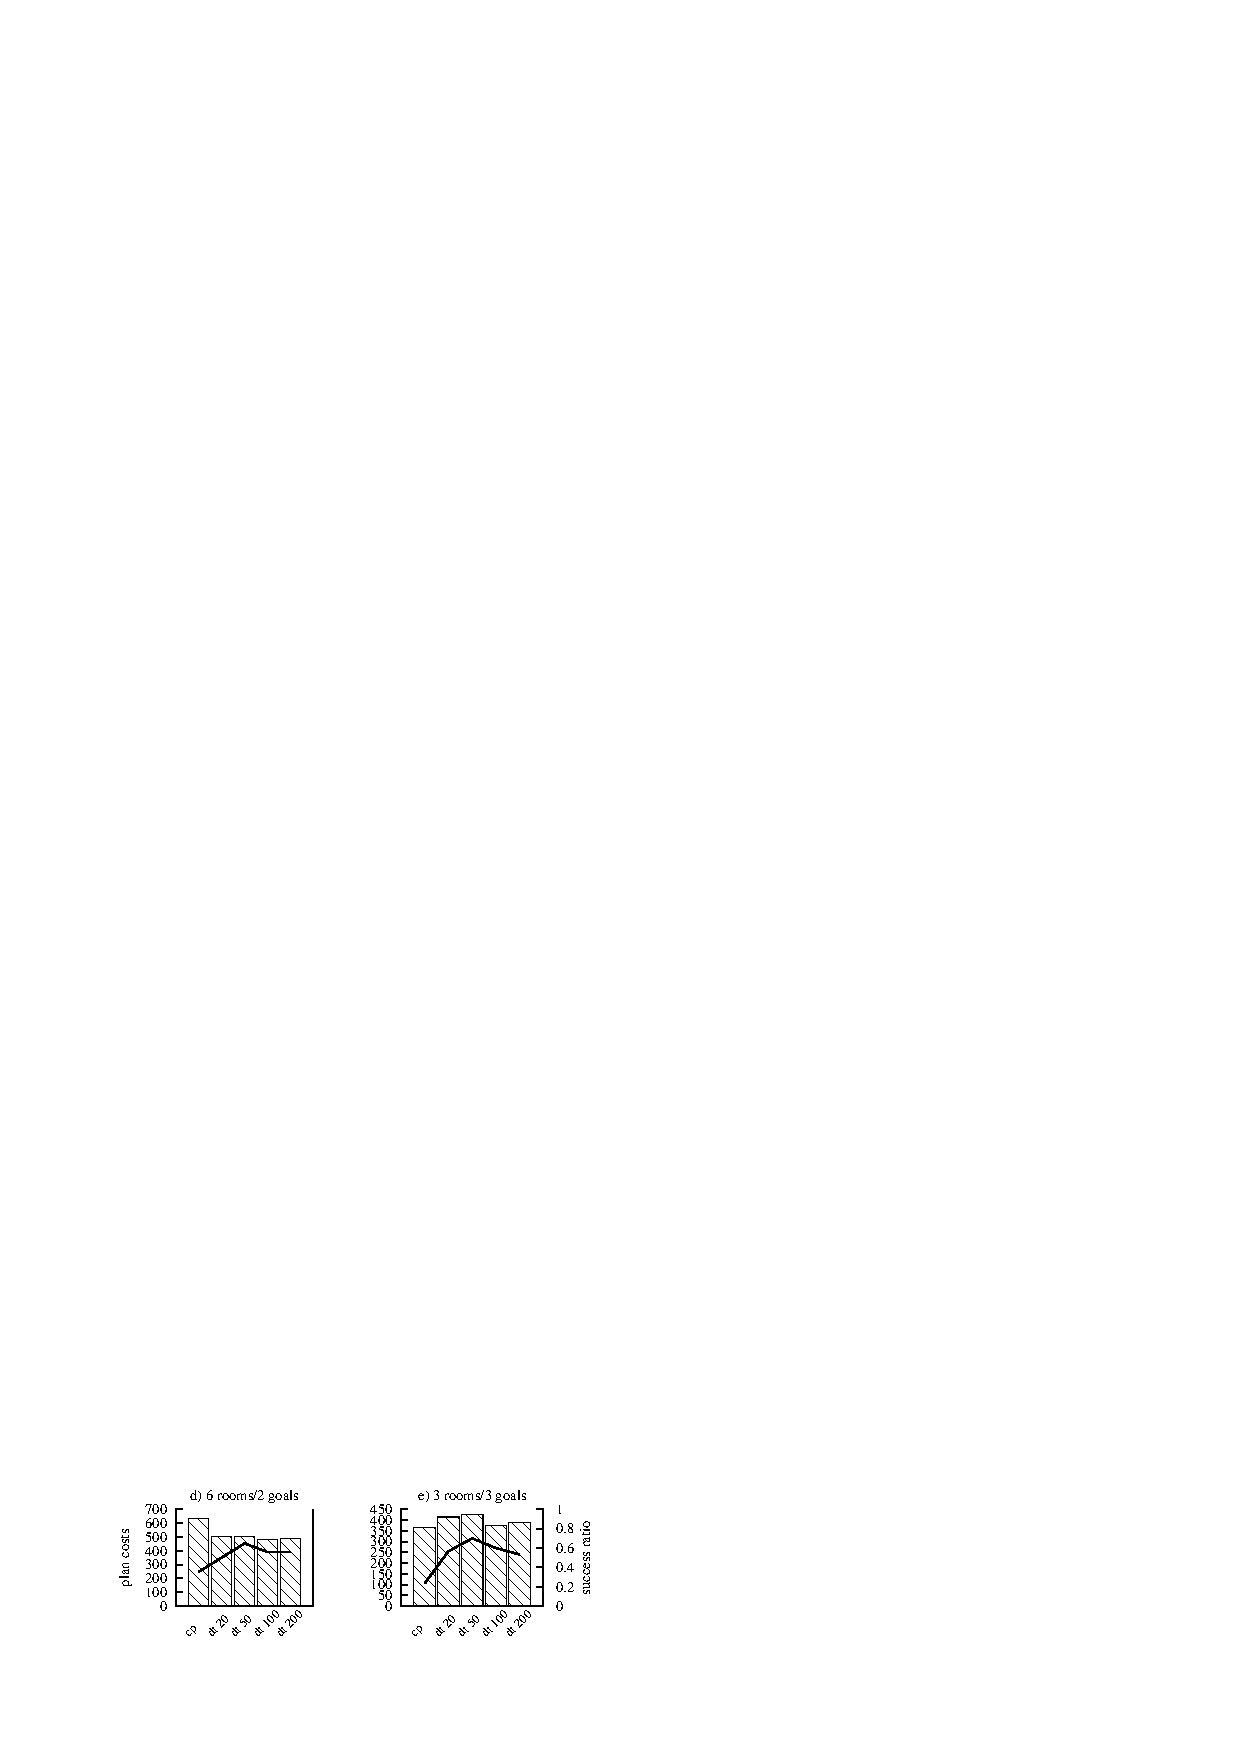
\includegraphics{dora56-quality}
  \caption{Average plan costs and number of successful runs}
  \label{fig:results-quality}
\end{figure}


The graphs in figure \ref{fig:results-time} show the average planning
times. For the smaller belief states, the cost for the decision
theoretic planning is compensated by the decrease of time spent in
Fast Downward.

Figure \ref{fig:results-quality} shows the average costs of the
executed plans as well as the percentage of solvable tasks that were
actually solved by the planner. For objects that can be easily
detected there is little gain in using a decision theoretic planner,
as the greedy sensing appoach by the baseline continual planner is
obviously sufficient here. With decreasing sensor reliability the more
sophisticated observation planning pays off: while the resulting plans
are still longer on average, the impact on the number of solved tasks
was much smaller than for the baseline system.

Impact of state space size: the configuration with a belief space size
of 200 was noticably slower than the other configurations while having
no noticable benefit. 

We believe that a part of the improvement is due to the segmentation of
the plan into several subtask, essentially performing hierarchical
planning. Especially when the continual planner performs badly this is
a huge gain.

%%% Local Variables: 
%%% mode: latex
%%% TeX-master: "moritz_2011"
%%% End: 
